\chapter[Analysis]{Analysis}

\section{Overview}
While Figure \ref{fig:alldata-GOES6-1983-1991} shows an overview of the most pertinent variables used in this study, some further analysis was done to determine any potential biases introduced by specifics of the satellite motion or derivations used. For example, where Figure \ref{fig:Takahashi2010Availability} shows that not only did data availability vary significantly with magnetic local time (MLT), Figure \ref{fig:ByHourExample} shows that the values themselves also vary significantly with MLT.  This leads to different models being better at particular times, such as AE models being better in the dawn sector and \dst\ models being better at dusk \citep{OBrien2003EmpiricalPlasmapause}. The concept of MLT having a strong effect on plasmospheric behavior has been well established all the way back to the initial whistler profiles of the plasmapause \citep{Carpenter1966WhistlerStudiesPlasmapause}.

\begin{figure}[htp!]
\centering
\includegraphics[width=0.7\linewidth]{Figures/rhoMLT.eps}
\caption{Median \req\ binned by magnetic local time.}
\label{fig:ByHourExample}
\end{figure}


\section{Linear Correlations}
This dependence was further investigated, and extended, by creating a simple linear model for each major variable in the database as well as combinations of some to investigate independent contributions to the total correlation (by testing how much correlation improved in a combined model over either of the constituent models.)  The inputs were the median values of each variable for four hours before a \dst\ event onset, and they were trained to predict a median of the value at onset with the four hours following it. The models were trained on half of the dataset and tested on the other half for each satellite, and this was repeated with new random samples 100 times and then the median correlation values were taken. The results are shown in Table \ref{CCperltable}.


\begin{table}[h]
	\small
	\caption{Table of linear model correlations showing the median of 100 random samples. Each sample trained on half of the data (via randomly selected rows of the least squares matrix) and tested on the other half.} 
 	\begin{tabular}{|C|CCCC|}
		\hline
		& \text{GOES 2} & \text{GOES 5} & \text{GOES 6} & \text{GOES 7}\\ \hline
		DoY & -0.08\pm0.08 & +0.14\pm0.13 & -0.06\pm0.06 & +0.09\pm0.10 \\
		MLT & -0.10\pm0.21 & -0.07\pm0.12 & +0.01\pm0.23 & -0.06\pm0.05 \\
		B_z & +0.16\pm0.21 & -0.13\pm0.15 & +0.08\pm0.14 & -0.07\pm0.06 \\
		V_{sw} & -0.04\pm0.10 & +0.27\pm0.09 & +0.06\pm0.11 & -0.06\pm0.06 \\
		D_{st} & +0.26\pm0.17 & +0.66\pm0.08 & +0.06\pm0.13 & +0.23\pm0.14 \\
		\rho_{sw} & +0.35\pm0.24 & +0.63\pm0.31 & +0.12\pm0.19 & +0.36\pm0.17 \\
		F_{10.7} & +0.43\pm0.08 & +0.12\pm0.12 & +0.51\pm0.06 & +0.40\pm0.06 \\
		B_z+V_{sw} & +0.11\pm0.17 & +0.20\pm0.17 & +0.12\pm0.10 & -0.12\pm0.06 \\
		D_{st}+F_{10.7} & +0.44\pm0.09 & +0.71\pm0.08 & +0.54\pm0.07 & +0.47\pm0.06 \\
		All & -0.03\pm0.19 & +0.34\pm0.27 & +0.61\pm0.11 & +0.40\pm0.12 \\
		\hline
	\end{tabular}
	\label{CCperltable}
\end{table}

 \begin{table}[h]
 	\small
 	\caption{Table of differences in linear training-testing models, where each correlation is the median correlation of 100 random samples. Each sample trained on half of the data (via randomly selected rows of the least squares matrix) and tested on the other half.} 
 	\begin{tabular}{|C|CCCC|}
 		\hline
 		Tr-T & \text{GOES 2} & \text{GOES 5} & \text{GOES 6} & \text{GOES 7}\\ \hline
 		DoY & +0.16\pm0.11 & +0.02\pm0.16 & +0.12\pm0.08 & -0.01\pm0.12 \\
 		MLT & +0.26\pm0.25 & +0.16\pm0.14 & +0.16\pm0.26 & +0.11\pm0.07 \\
 		B_z & +0.06\pm0.24 & +0.27\pm0.18 & +0.05\pm0.17 & +0.14\pm0.08 \\
 		V_{sw} & +0.11\pm0.13 & +0.02\pm0.13 & +0.03\pm0.13 & +0.12\pm0.08 \\
 		D_{st} & +0.02\pm0.21 & +0.01\pm0.12 & +0.06\pm0.16 & +0.00\pm0.17 \\
 		\rho_{sw} & +0.01\pm0.29 & +0.01\pm0.37 & +0.04\pm0.22 & -0.03\pm0.21 \\
 		F_{10.7} & -0.01\pm0.11 & +0.04\pm0.16 & +0.00\pm0.08 & +0.03\pm0.08 \\
 		B_z+V_{sw} & +0.15\pm0.20 & +0.17\pm0.20 & +0.08\pm0.12 & +0.24\pm0.08 \\
 		D_{st}+F_{10.7} & +0.05\pm0.12 & -0.02\pm0.11 & +0.01\pm0.10 & +0.03\pm0.08 \\
 		All & +0.64\pm0.22 & +0.54\pm0.28 & +0.16\pm0.14 & +0.25\pm0.13 \\
 		\hline
 	\end{tabular}
 	\label{CCdifftable}
 \end{table}



It can be seen that $F_{10.7}$ almost always correlates the best with \req, but that there is significant variance between data from different satellites. \dst\ also tends to correlate well, but when making a linear model that combines both \f\ and \dst, not much improvement is gained suggesting a high degree of collinearity between the two. 

Table \ref{CCdifftable} shows the difference between the correlation values for the training set and the test set. This is intended to show which variables are more susceptible to overfitting, since they would tend to correlate well with the training set but not the test set and end up having a large difference. The variables that had good test correlation (\f\  and \dst) also had small differences, indicating they were actually good predictors. The models that benefited from an abundance of data to fit (such as using all variables), or those that had a simple linear structure easy to fit to anything ($DoY$ and $MLT$), had large differences due to being highly overfit to the training set. 

\section{Nonlinear Correlations}

Similarly for a neural net model with the same input and target structure as the linear model, but training on a randomly selected 70\% of the data, testing on another 15\%, and validating on the remaining 15\%, Table \ref{NNperltable} shows the resulting correlation values for the validation data set.

 \begin{table}[h]
 	\small
 	\caption{Table of nonlinear model test correlations showing the median of 100 random samples. Each sample trained on half of the data (via randomly selected rows of the least squares matrix) and tested on the other half.} 
 	\begin{tabular}{|C|CCCC|}
 		\hline
 		& \text{GOES 2} & \text{GOES 5} & \text{GOES 6} & \text{GOES 7}\\ \hline
 		DoY & +0.05\pm0.31 & +0.31\pm0.30 & +0.32\pm0.22 & +0.12\pm0.17 \\
 		MLT & +0.29\pm0.41 & +0.15\pm0.34 & +0.40\pm0.32 & +0.17\pm0.21 \\
 		B_z & +0.24\pm0.23 & +0.21\pm0.28 & +0.17\pm0.19 & -0.00\pm0.20 \\
 		V_{sw} & +0.20\pm0.25 & +0.36\pm0.19 & +0.19\pm0.24 & +0.06\pm0.18 \\
 		D_{st} & +0.08\pm0.27 & +0.18\pm0.25 & +0.02\pm0.17 & +0.18\pm0.24 \\
 		\rho_{sw} & +0.02\pm0.29 & +0.25\pm0.42 & +0.20\pm0.22 & +0.12\pm0.29 \\
 		F_{10.7} & +0.26\pm0.27 & +0.32\pm0.29 & +0.48\pm0.25 & +0.36\pm0.15 \\
 		B_z+V_{sw} & +0.11\pm0.25 & +0.20\pm0.38 & +0.15\pm0.21 & +0.02\pm0.17 \\
 		D_{st}+F_{10.7} & +0.17\pm0.25 & +0.21\pm0.32 & +0.47\pm0.15 & +0.35\pm0.17 \\
 		All & +0.21\pm0.41 & +0.67\pm0.40 & +0.60\pm0.35 & +0.17\pm0.33 \\
 		\hline
 	\end{tabular}
 	\label{NNperltable}
 \end{table}
 
 
 
 \begin{table}[h]
 	\small
 	\caption{Table of differences in nonlinear training-testing models, where each correlation is the median correlation of 100 random samples. Each sample trained on half of the data (via randomly selected rows of the least squares matrix) and tested on the other half.} 
 	\begin{tabular}{|L|LLLL|}
 		\hline
 		Tr-T & \text{GOES 2} & \text{GOES 5} & \text{GOES 6} & \text{GOES 7}\\ \hline
 		DoY & +0.48\pm0.36 & +0.17\pm0.33 & +0.18\pm0.24 & +0.27\pm0.23 \\
 		MLT & +0.31\pm0.40 & +0.28\pm0.42 & +0.31\pm0.36 & +0.28\pm0.26 \\
 		B_z & +0.14\pm0.27 & +0.29\pm0.33 & +0.20\pm0.27 & +0.20\pm0.19 \\
 		V_{sw} & +0.27\pm0.31 & +0.22\pm0.31 & +0.20\pm0.27 & +0.24\pm0.19 \\
 		D_{st} & +0.37\pm0.32 & +0.27\pm0.32 & +0.18\pm0.21 & +0.21\pm0.24 \\
 		\rho_{sw} & +0.31\pm0.30 & +0.16\pm0.42 & +0.24\pm0.27 & +0.47\pm0.37 \\
 		F_{10.7} & +0.19\pm0.28 & +0.19\pm0.29 & +0.15\pm0.25 & +0.18\pm0.26 \\
 		B_z+V_{sw} & +0.28\pm0.31 & +0.26\pm0.32 & +0.28\pm0.22 & +0.23\pm0.19 \\
 		D_{st}+F_{10.7} & +0.30\pm0.29 & +0.20\pm0.32 & +0.14\pm0.19 & +0.20\pm0.16 \\
 		All & +0.51\pm0.58 & +0.47\pm0.60 & +0.41\pm0.36 & +0.46\pm0.43 \\
 		\hline
 	\end{tabular}
 	\label{NNdifftable}
 \end{table}

 

It should be noted that nonlinear modeling is generally more susceptible to overfitting than linear modeling due to the higher order of fitting done on training and validation data, the use of more fit parameters for similarly structured models,  as well as the lack of a straight-forward optimal error-minimization method such as least squares regression. This is why some models, such as that including every possible variable, correlate worse than models of just a few parts. Where a linear model can minimize error by zeroing out variables without useful information, the neural net will try to incorporate the information anyway and end up overfitting. Table \ref{NNdifftable} shows how significant the differences are between training data and testing data by subtracting the median correlations from both data sets from each other, and doing the root mean squared (RMS) error as the combination of the two constituent errors.

\section{ARX}
In an effort to combine the usefulness of linear models with the adaptability of nonlinear models, a number of ARX models were made to find if they could predict \req\ given variables over a number of time lags as input. Two forms were made: one with a 1-hour time lag, essentially a normal linear model predicting \req\ using each variable, and one with 24 hours of lags for each included variable. Each model would generate a matrix of the form shown in Chapter 2, boostrap sample all the rows 100 times generating a set of ARX coefficients each time, the take the mean of those coefficients for the model used to reconstruct the target timeseries. The correlation between this reconstruction and the target is then printed to a table, a subset of which is shown in Table \ref{ARXTable}.

 \begin{table}[h]
 	\small
 	 	\caption{Table of ARX model correlations created from the mean of 100 bootstrap models. CC-1 models have one hour of time lag, and CC-24 have 24 hours of time lags.} 
 	\begin{tabular}{|C|CC|}
 		\hline
 		& \text{CC-1} & \text{CC-24} \\ \hline
 		DoY & +0.02 & +0.04 \\
 		Hour & +0.07 & +0.27 \\
 		B_z & +0.14 & +0.22 \\
 		V_{sw} & +0.20 & +0.21\\
 		D_{st} & +0.03 & +0.05\\
 		K_p & +0.10 & +0.10 \\
 		\rho_{sw} & +0.07 & +0.08 \\
 		F_{10.7} & +0.43 & +0.45 \\
 		B_z+V_{sw} & +0.24 & +0.29 \\
 		B_z+Hour & +0.16 & +0.32 \\
 		B_z+F_{10.7} & +0.45 & +0.49 \\
 		Hour+F_{10.7} & +0.44 & +0.48 \\
 		D_{st}+F_{10.7} & +0.44 & +0.46 \\
 		All & +0.56 & +0.61 \\
 		\hline
 	\end{tabular}
 	\label{ARXTable}
 \end{table}


It is interesting to note which variables correlate just as well on an hourly timescale as on a daily timescale (e.g. \f) compared to those which show significant improvement as more time is added to the model (e.g. Hour). The collinearity of some models is also interesting, such as how adding an hourly component does not aid the \f\ model much, but does significantly help the $B_z$ model. Also, adding one hour of persistence to the model increases the correlation to $0.88-0.91$ for all of the models. 


\section{Epoch Analyses} \label{sec:epochs}
In an effort to determine the typical behavior of an event, analyses were done for a number of different conditions where all variables were averaged over a window surrounding the event onset. This should reduce the noise of individual events and show the overall trends inherent in the system during different types of events. For example, Figure \ref{fig:EpochDst} shows the data for \dst\ events where \dst\ dropped below $-50$~nT. This finds 333 such events over the span of time covered by GOES 6. Taking the median of each variable across all events for each time step (an hour, in this figure), the general trend is plotted for $B_z$, $V_{SW}$, \dst,\f, and \req. The red dashed lines indicate one standard error of the mean from all of the valid points used to compute the median, and the number of valid points (relevant only for \req) is plotted as green bars.

\begin{figure}[htp!]
	\centering
	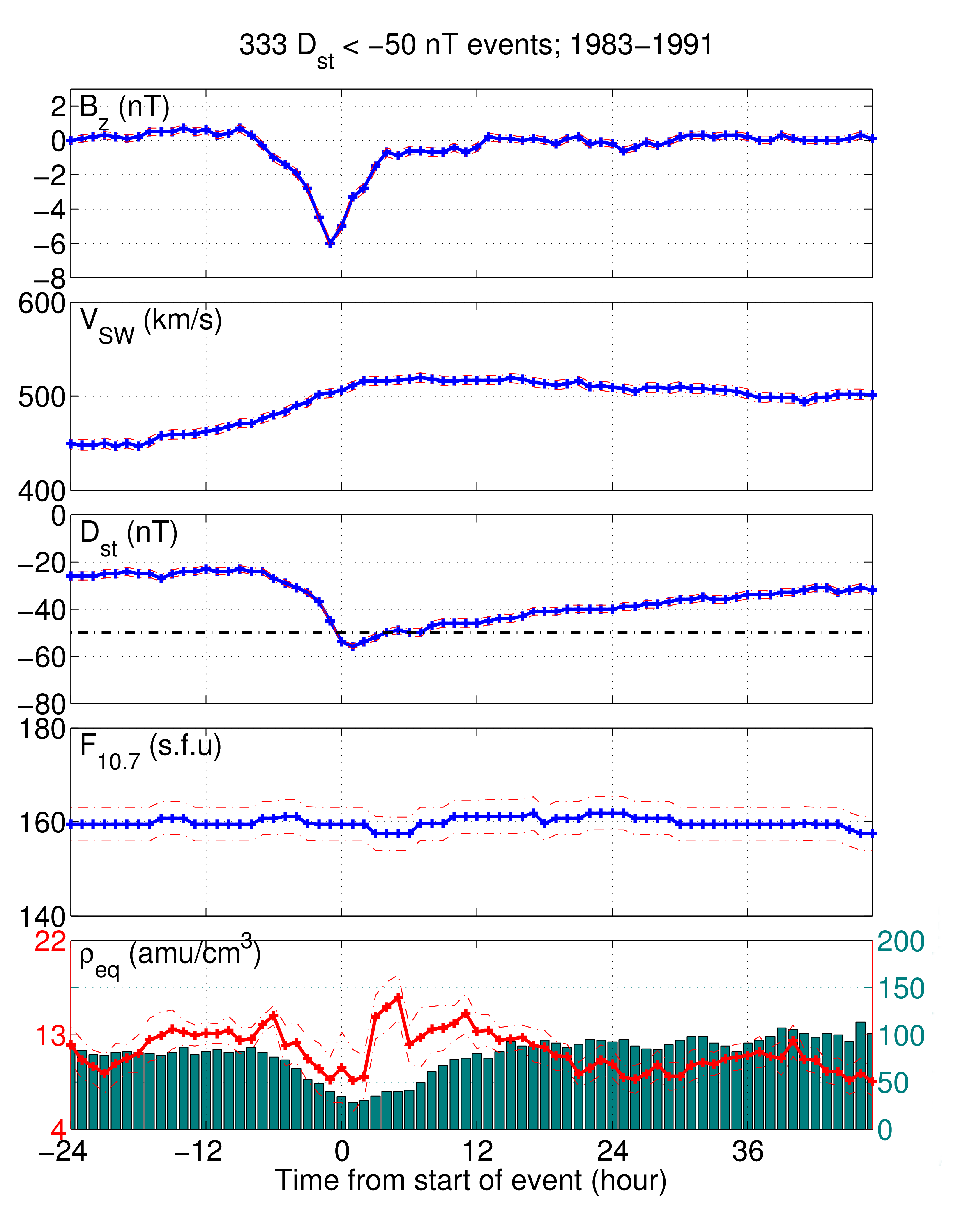
\includegraphics[width=1\linewidth]{Figures/StormAvs/stormavs-dst-GOES6}
	\caption{Epoch analysis for \dst\ events on an hourly timescale.}
	\label{fig:EpochDst}
\end{figure}

Figure \ref{fig:EpochDst} shows that a \dst\ decrease is, on average and with little variation, preceded by a large drop in $B_z$, a slightly faster solar wind, and a spike in \req. To see if there were also significant changes over a longer period, the same analysis was done after binning all data to a daily time scale, and the results are shown in Figure \ref{fig:EpochDstDay}.

\begin{figure}[htp!]
	\centering
	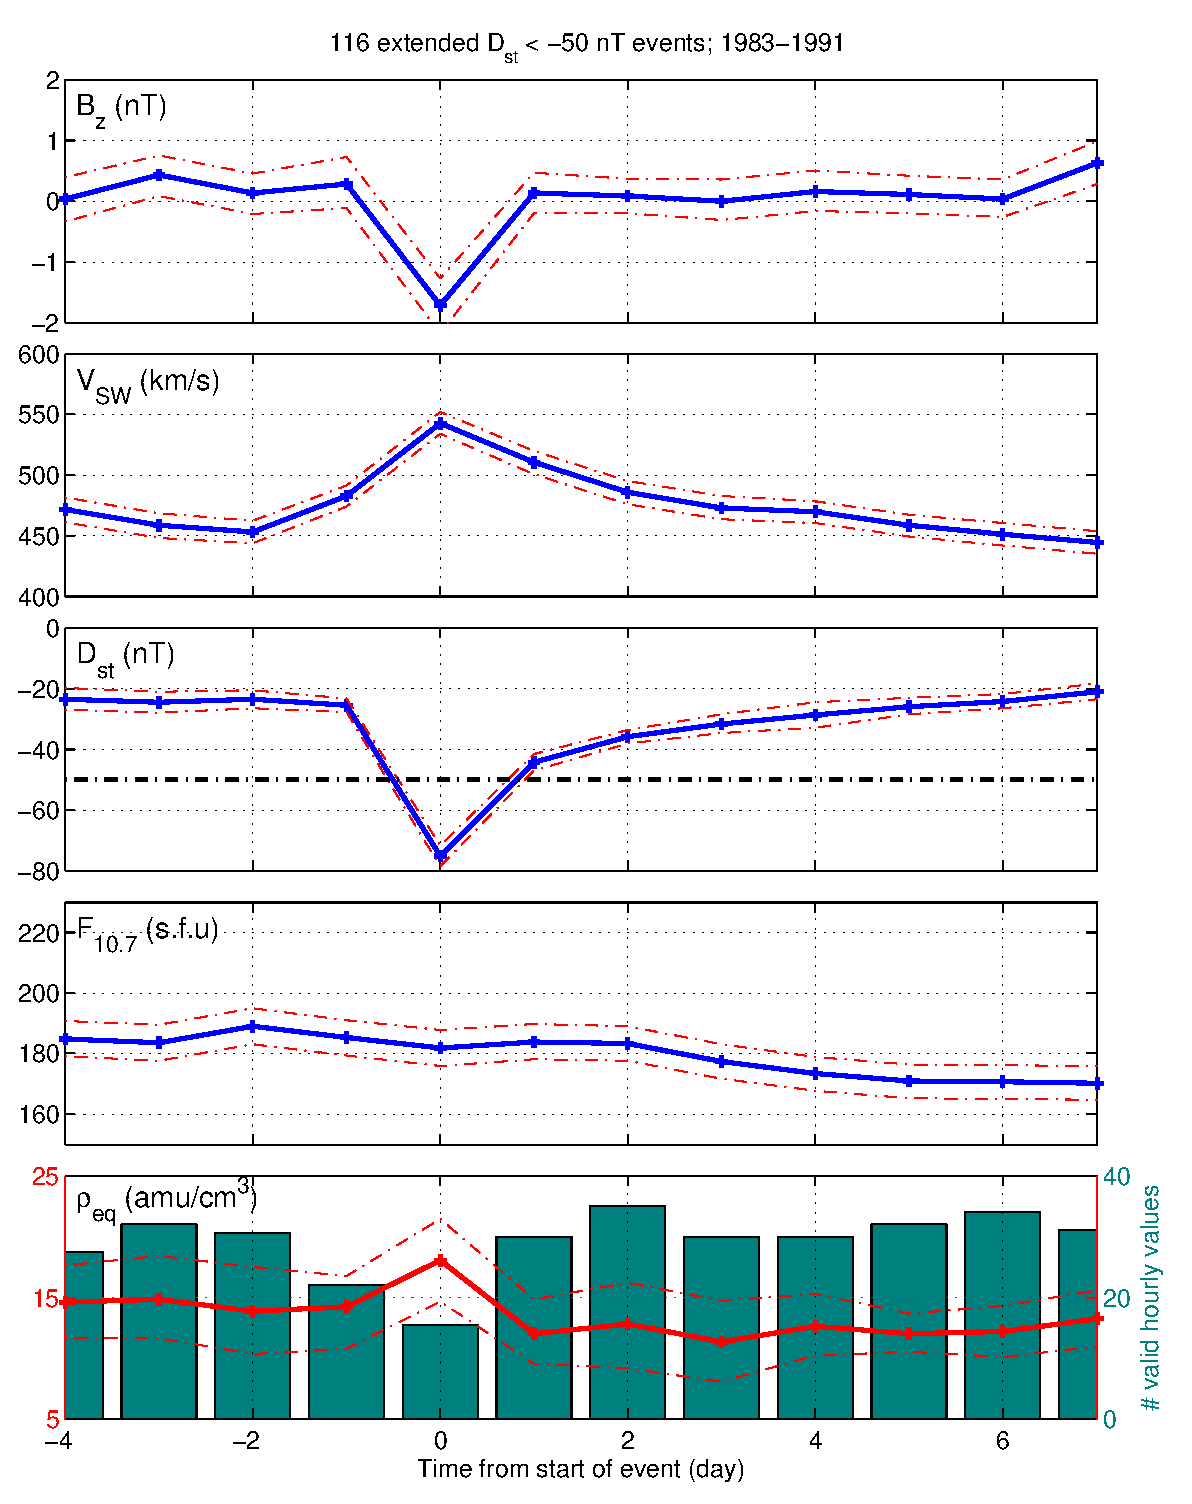
\includegraphics[width=1\linewidth]{Figures/StormAvs/stormavs-dst-day-GOES6}
	\caption{Epoch analysis for \dst\ events on an daily timescale.}
	\label{fig:EpochDstDay}
\end{figure}

This shows the same decrease of $B_z$ accompanying a decrease in \dst, but also more clearly shows that the solar wind velocity and \req\ both also differ significantly from the day before onset to onset (in the case of velocity) and the day of onset to the day after (in the case of density). 

In an effort to replicate the results of \cite{Takahashi2010SolarCycleVariation}, shown in Figure \ref{fig:EpochTakahashi}, the same epoch analysis was done on a daily timescale for just the years looked at in the paper (1989-1991), and a similar plot was created. This is shown in Figure \ref{fig:EpochDstDayTakahashi}, and finds results that are fairly similar, with slight differences possibly attributable to difference in data pruning. \cite{Takahashi2010SolarCycleVariation} only looks at events happening between 0600 and 1200 MLT since their $f_{T3}$ detection rate was highest then and also defines "onset" as time corresponding to the minimum value in an event where \dst\ crossed the $-50$~nT threshold. These adjustments  were added to this analysis to both verify the results of \cite{Takahashi2010SolarCycleVariation}, and verify that the data handling and analysis routines being used were accurate and repeatable with respect to the results from other researchers.

\begin{figure}[htp!]
	\centering
	\includegraphics[width=0.7\linewidth]{Figures/StormAvs/stormavs-Takahashi.png}
	\caption{Epoch analysis for \dst\ events on an daily timescale using only the years of 1989-1991 from \citep{Takahashi2010SolarCycleVariation}.}
	\label{fig:EpochTakahashi}
\end{figure}

\begin{figure}[htp!]
	\centering
	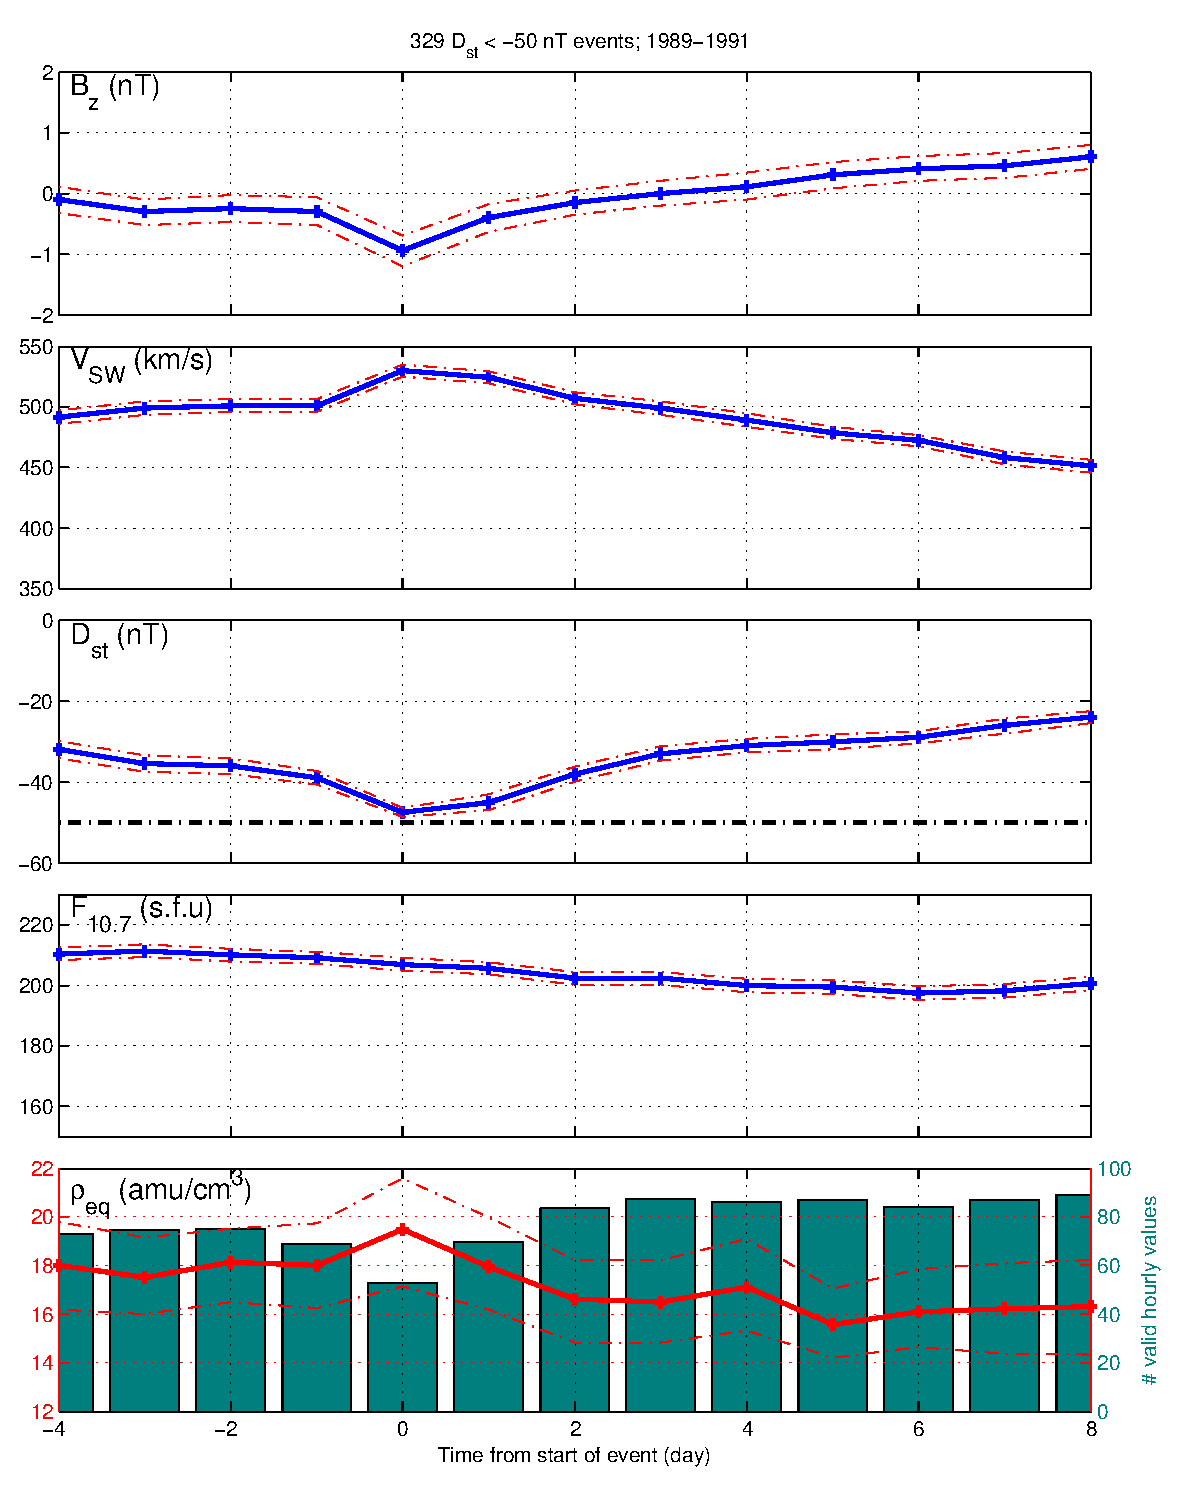
\includegraphics[width=1\linewidth]{Figures/StormAvs/stormavs-dst-50-tak-GOES6}
	\caption{Epoch analysis for \dst\ events on an daily timescale using only the years of 1989-1991.}
	\label{fig:EpochDstDayTakahashi}
\end{figure}



To verify that there was in fact a significant difference between the day of onset and the day to either side, a bootstrap significance test was performed where a number of samples equal to the number of events was selected at random with replacement, and the median values were calculated. This was done 1000 times, and a histogram was created showing the distribution of differences between median values, shown in Figure \ref{fig:DailyBootstrapDifferences}

\begin{figure}[htp!]
	\centering
	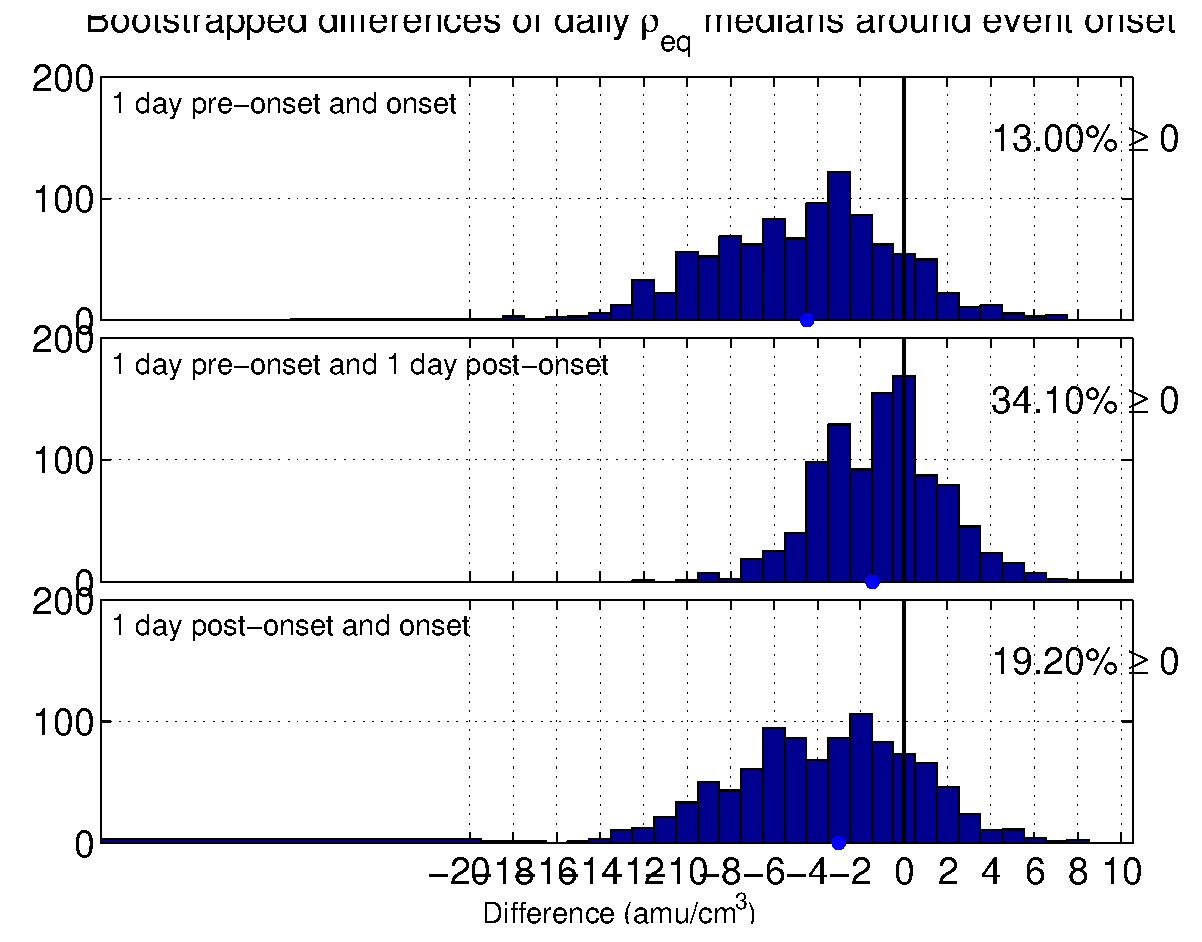
\includegraphics[width=1\linewidth]{Figures/DailyBootstrapDifferences-GOES6-case10}
	\caption{Bootstrap differences between median daily value of events using only the years of 1989-1991.}
	\label{fig:DailyBootstrapDifferences}
\end{figure}


The idea here is that if the days have equal medians, a large number of random samples for each day should be equal on average. If the medians of two days are equal, the difference between those medians should be zero, so if a significant portion of differences have a skewed to non-zero value, this suggests the days are not equal. Figure \ref{fig:DailyBootstrapDifferences} shows that for the time period of 1989-1991, no significance can be conclusively shown in this manner. Looking the entirety of data from GOES 6, covering 1983-1991, as seen in Figure \ref{fig:DailyBootstrapDifferences-full}, this trend remains similar in distributions.  

\begin{figure}[htp!]
	\centering
	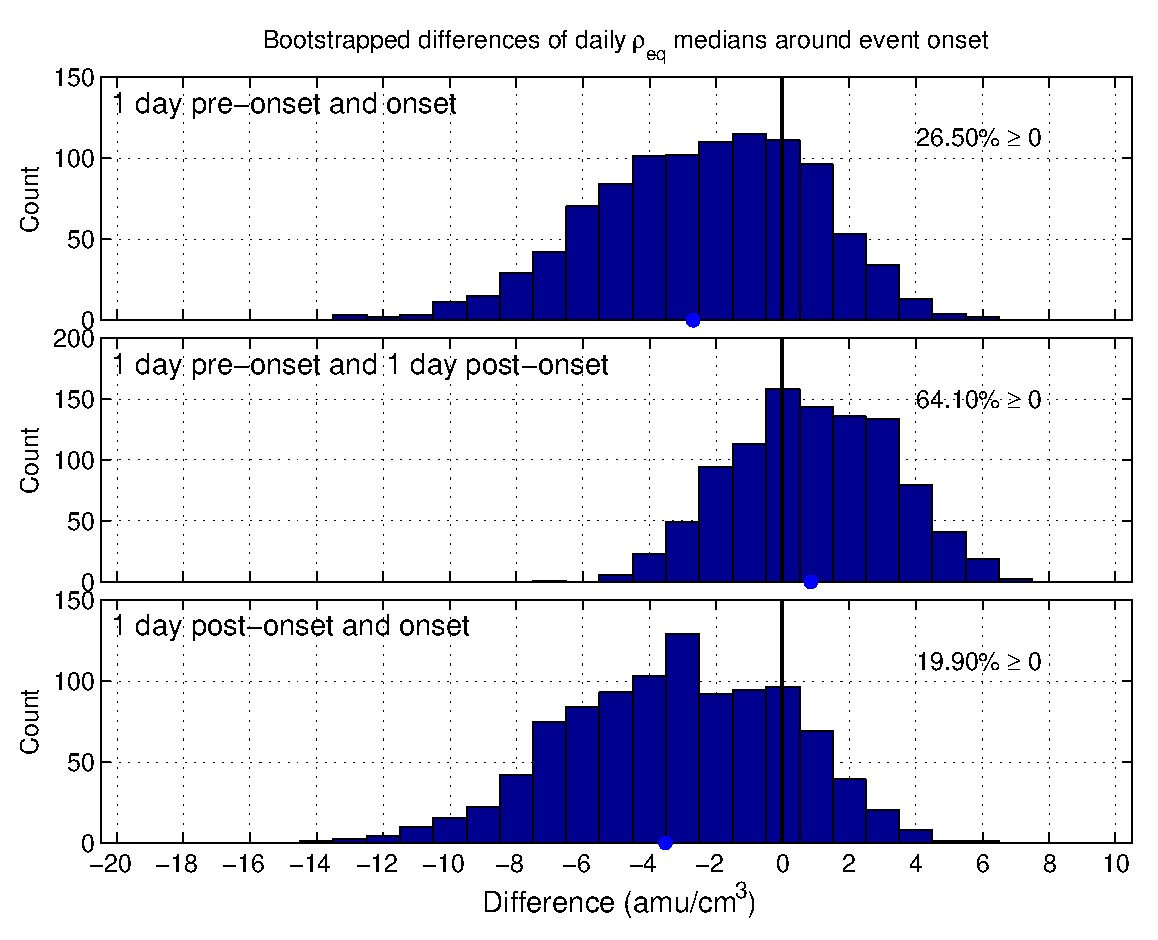
\includegraphics[width=1\linewidth]{Figures/DailyBootstrapDifferences-GOES6-case13}
	\caption{Bootstrap differences between median daily value of events using the years of 1983-1991.}
	\label{fig:DailyBootstrapDifferences-full}
\end{figure}

A few other forms of epoch analysis were done for exploratory purposes. Figure \ref{fig:EpochDst12Hour} shows \dst\ events where \dst\ remained below the $-50$~nT threshold for at least 12 hours. The same preceding drop in $B_z$ can be seen, but now also appears to sustain the more negative value for longer. Also of note is the large spike in \req, but it comes at a point with few available data points, and the uncertainty on each point is large, making it difficult to say anything conclusive about the behavior of density during sustained periods of highly negative \dst other than that it follows the general trend of hourly \req\ increases in response to geomagnetic activity.

\begin{figure}[htp!]
	\centering
	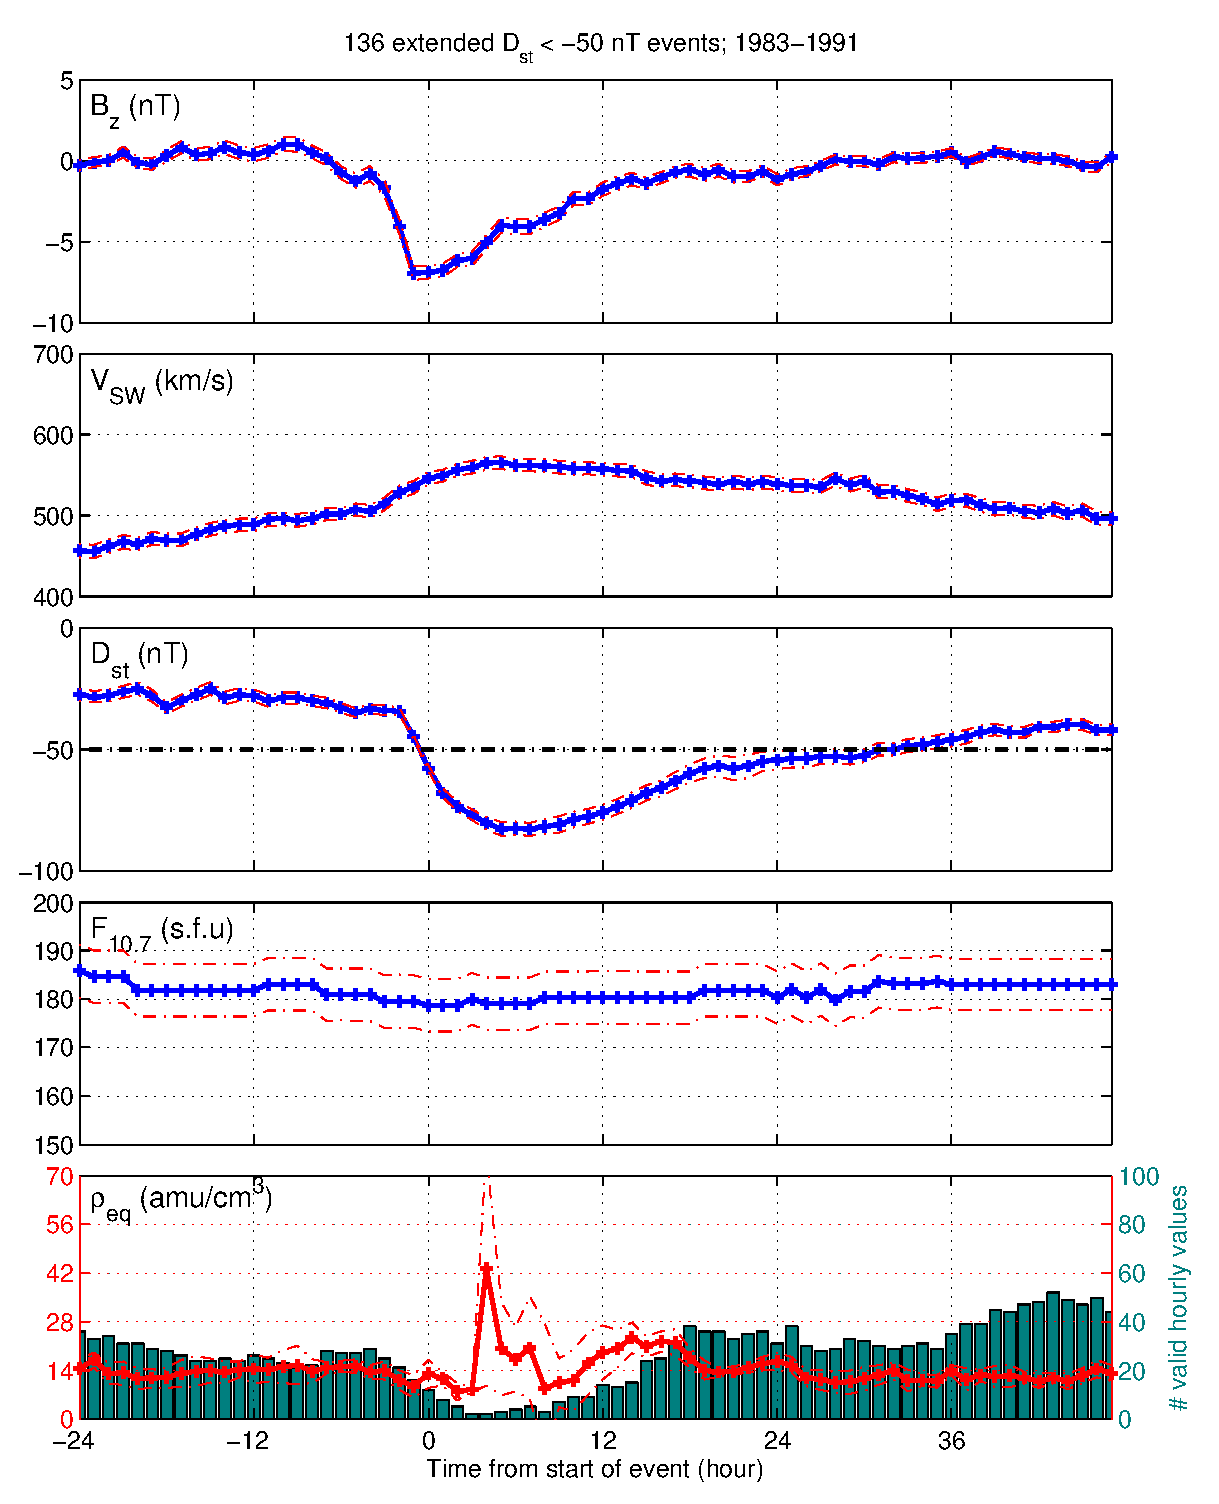
\includegraphics[width=1\linewidth]{Figures/StormAvs/stormavs-dd12-GOES6}
	\caption{Epoch analysis for \dst\ events lasting longer than 12 hours.}
	\label{fig:EpochDst12Hour}
\end{figure}

Looking at events defined as a period where \req\ crosses a threshold of 20 $amu/cm^3$ shows, in Figure \ref{fig:EpochRho}, that there are no apparent trends in the solar wind or solar variables coinciding with the increase in density.

\begin{figure}[htp!]
	\centering
	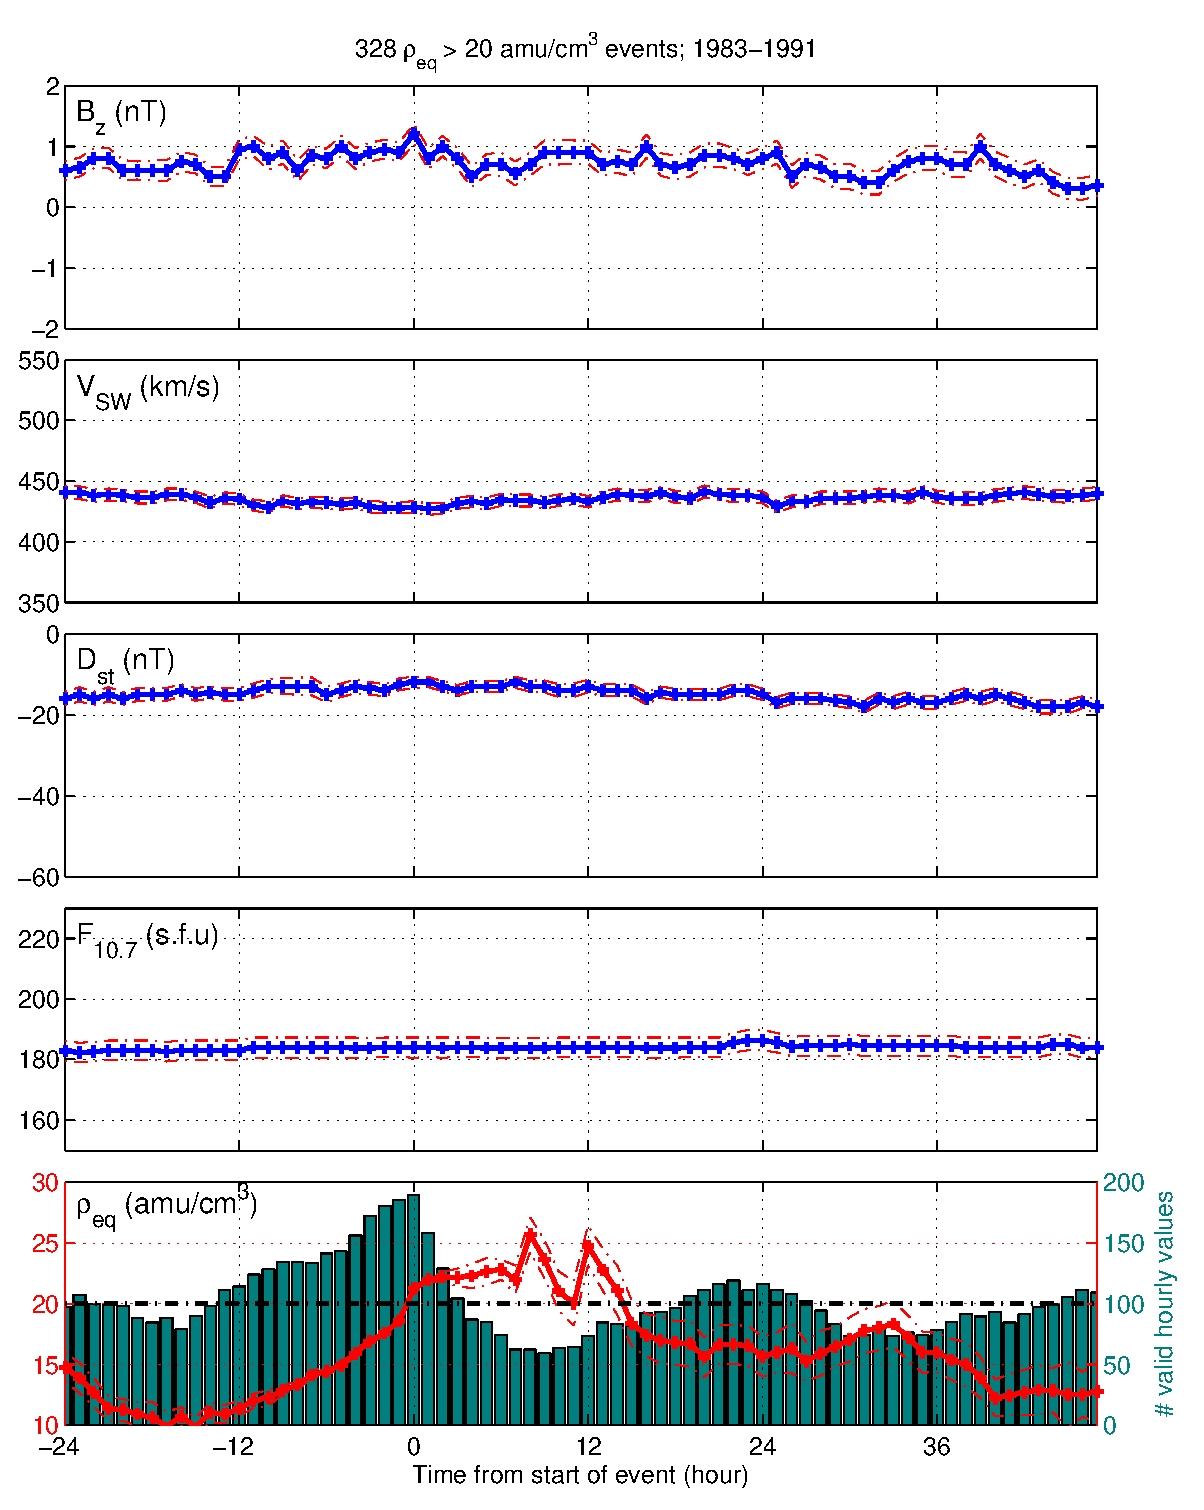
\includegraphics[width=1\linewidth]{Figures/StormAvs/stormavs-mass-gt20-GOES6}
	\caption{Epoch analysis for \req\ events on an hourly timescale.}
	\label{fig:EpochRho}
\end{figure}

And finally, to test the amount of natural variance and for the sake of verification, a stack plot was made with random times selected as event onsets for both hourly and daily data. Figure \ref{fig:EpochRandom} shows the hourly example, and neither have any significant trends, as expected.

\begin{figure}[htp!]
	\centering
	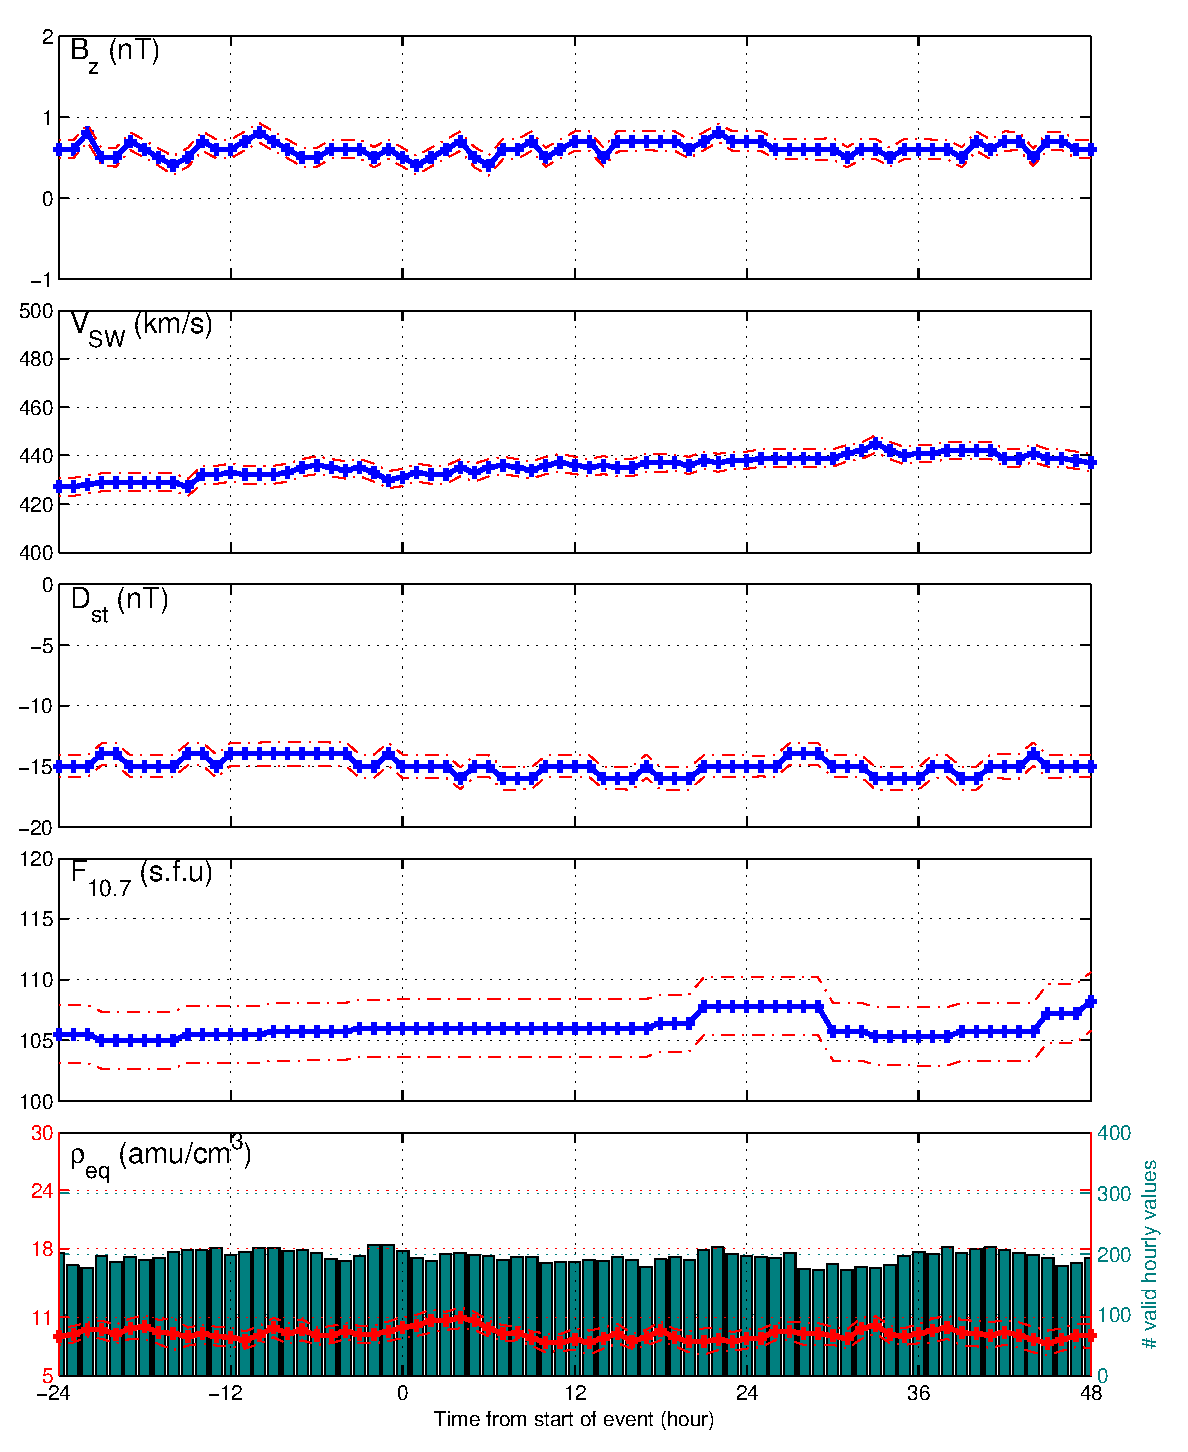
\includegraphics[width=1\linewidth]{Figures/StormAvs/stormavs-random-GOES6}
	\caption{Epoch analysis for randomly selected "events" between 1983-1991 on an hourly timescale.}
	\label{fig:EpochRandom}
\end{figure}

\clearpage



\section{$F_{10.7}$ Dependence} \label{sec:f107dep}
\cite{Takahashi2010SolarCycleVariation} showed a strong correlation between the 27-day averaged $F_{10.7}$ index of solar activity and the averaged equatorial mass density (\req). This was chosen as a starting place for verifying the data analysis routines developed for this dataset, so as to show that data input, averaging, and interpolation were all done in a reasonable and reproducible manner. Figure \ref{fig:F107rhoeq27dcomparison} shows the strong correlation seen previously, and reasonably reproduces Figure 13.b from \cite{Takahashi2010SolarCycleVariation} for the years covered by GOES 6. Figure \ref{fig:ccplot} shows the effects of long-time-scale averaging on the overall correlation of the two variables, suggesting that the connection is more influential long-term.

\begin{figure}[htp!]
	\centering
	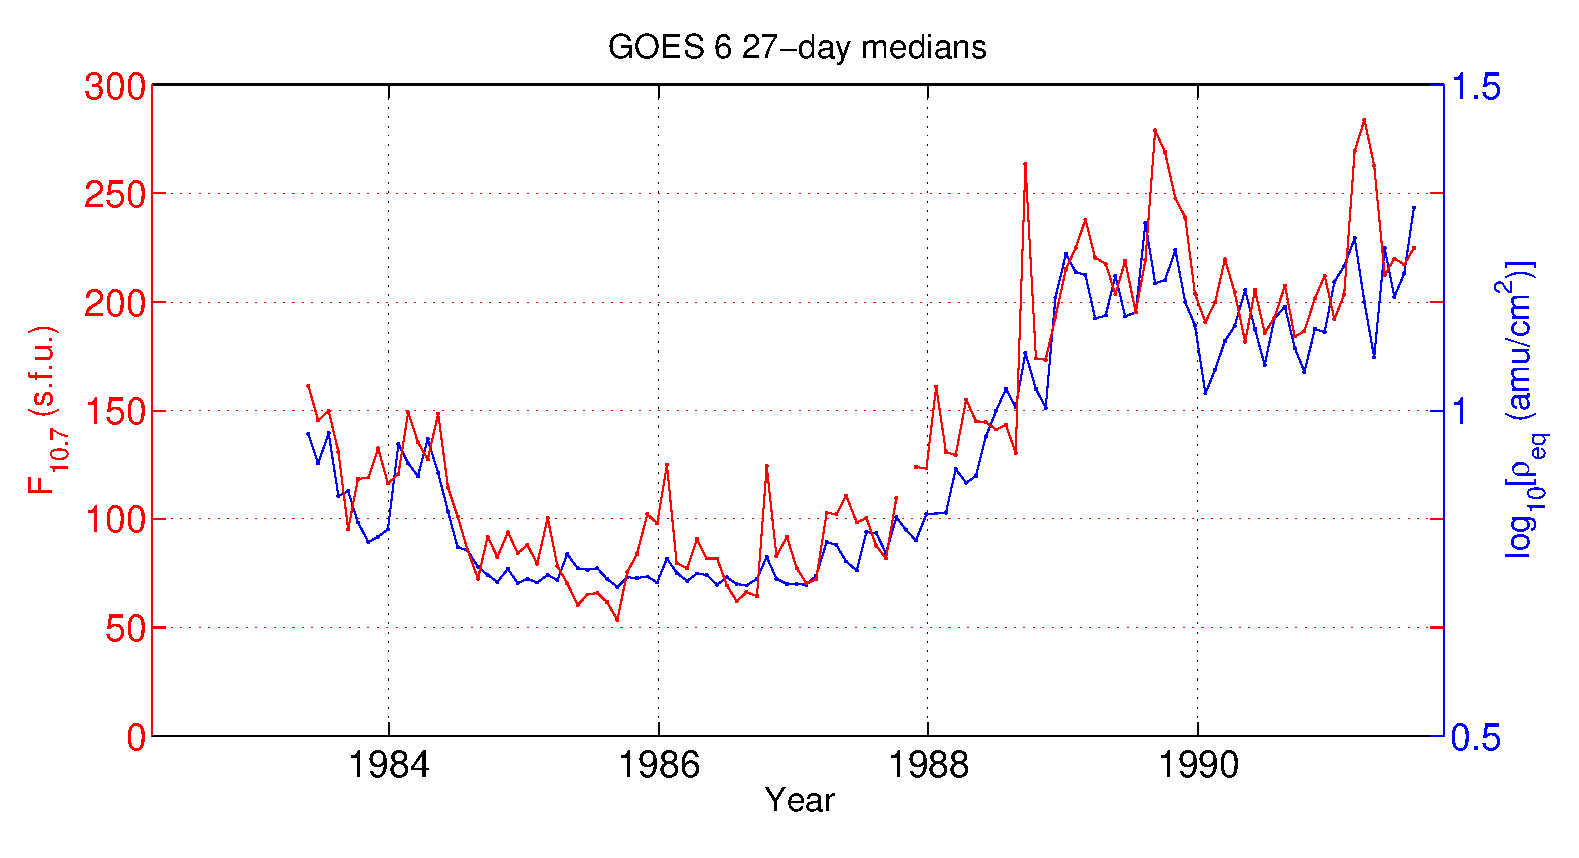
\includegraphics[width=0.95\linewidth]{Figures/F107MD27d-GOES6}
	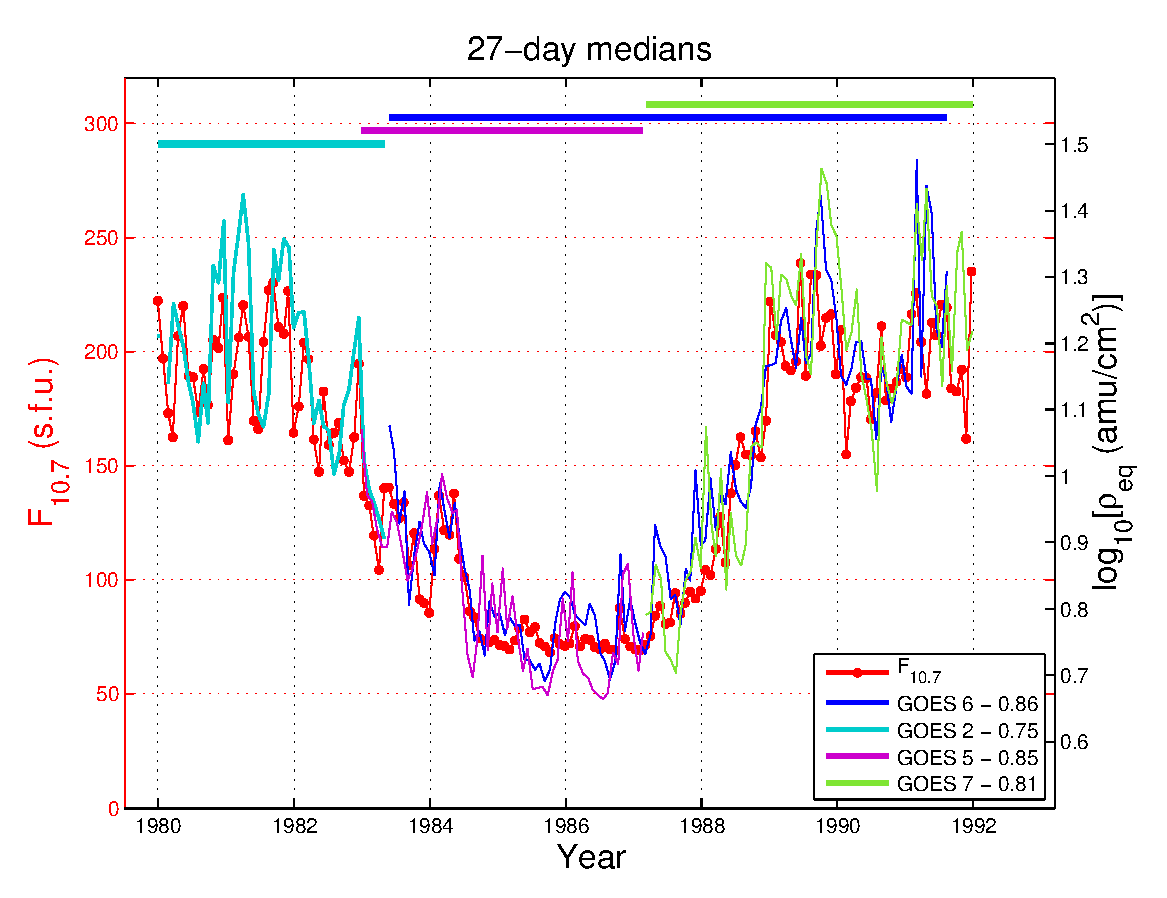
\includegraphics[width=0.95\linewidth]{Figures/F107MD27d-all}
	\caption{Top: Comparing $F_{10.7\_27d}$ and $\log_{10}(\rho_{eq\_27d})$ using GOES 6 data. Bottom: Same as top, but all available satellites.}
	\label{fig:F107rhoeq27dcomparison}
\end{figure}

\begin{figure}[htp!]
	\centering
	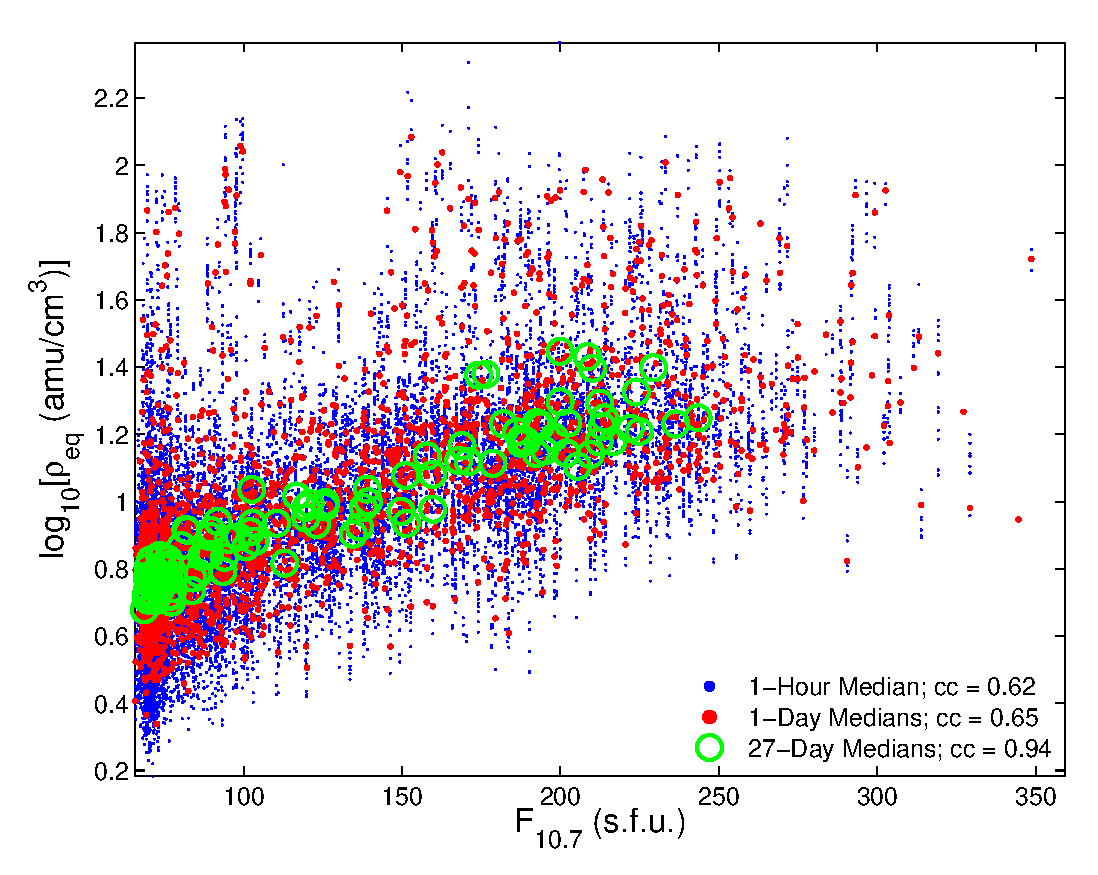
\includegraphics[width=0.7\linewidth]{Figures/ccplot-GOES6}
	\caption{\f\ and $log(\req)$ correlation at varying time scales.}
	\label{fig:ccplot}
\end{figure}


The dependence was then analyzed in a more nonlinear manner by investigating the behavior of storms under different $F_{10.7}$ conditions. The hypothesis being that solar activity would drive both geomagnetic storms and, consequently, \req. By separating storms into bins based on the median value of \f, then breaking those two bins into another two bins each separated by their respective medians, a profile of all storm behavior based on \f\ is obtained. Figure \ref{fig:HighLowF107rhoeq} shows the results of this across the events where \dst\ crossed below the $-50$~nT threshold. 

\begin{figure}[htp!]
	\centering
	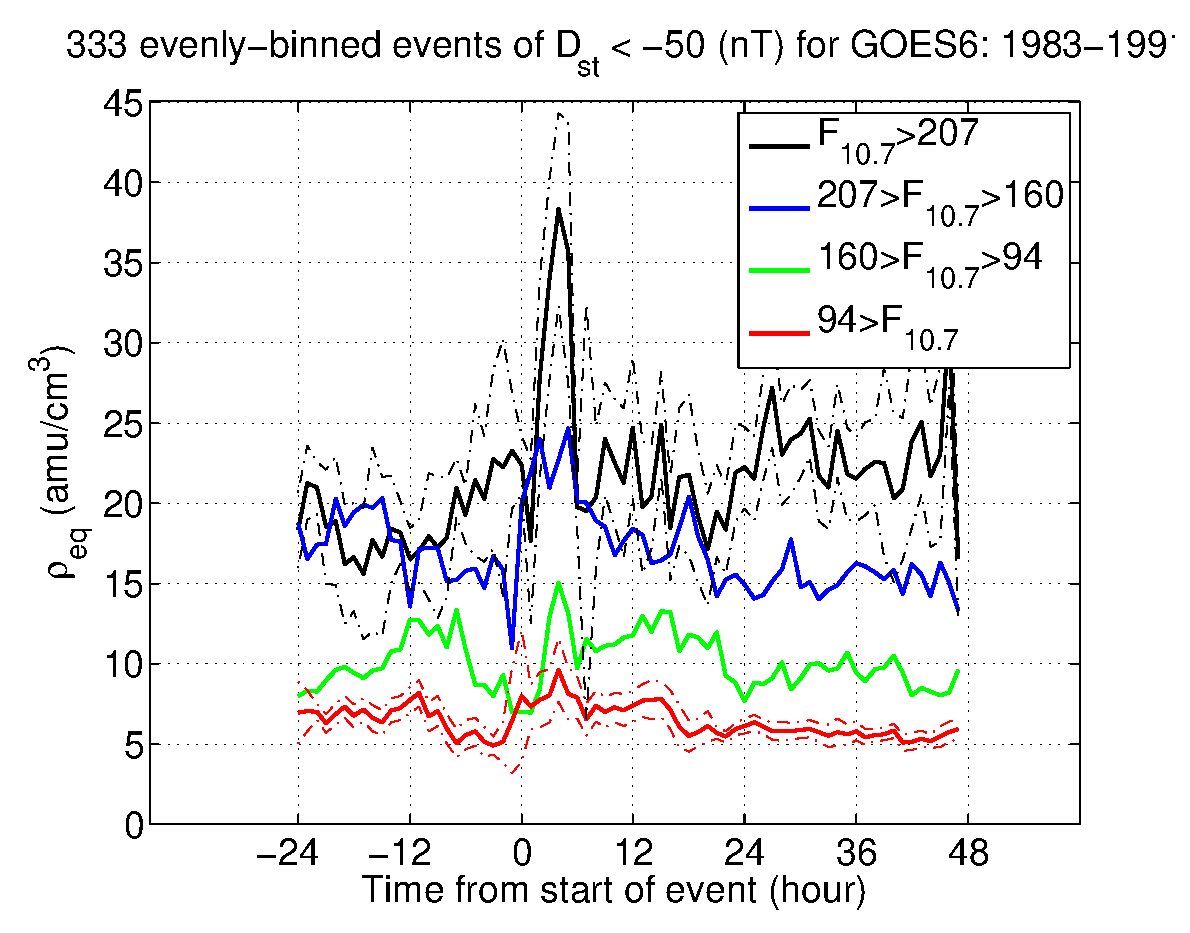
\includegraphics[width=0.7\linewidth]{Figures/HighLowF107rhoeq-Dst50-GOES6-1983-1991}
	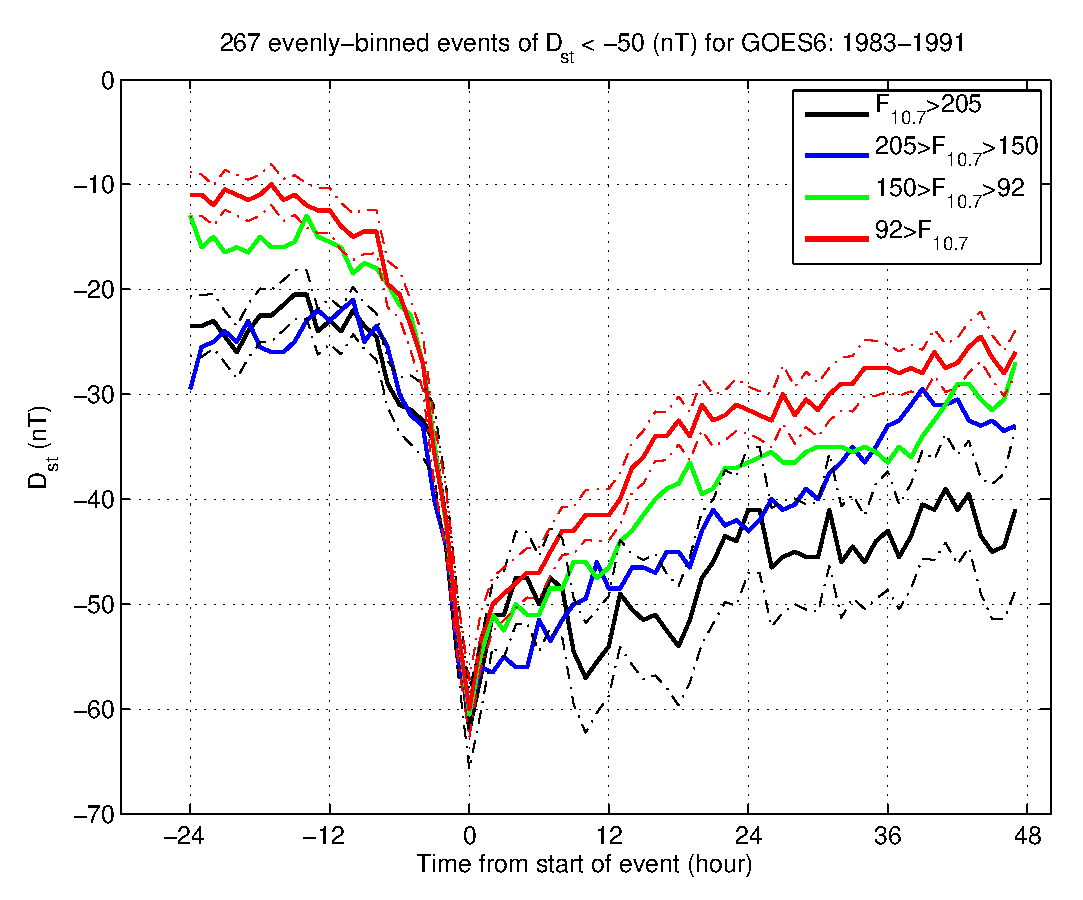
\includegraphics[width=0.7\linewidth]{Figures/HighLowF107Dst-Dst50-GOES6-1983-1991}	
	\caption{\req\ (top panel) and \dst\ (bottom panel) of \dst\ events binned by median \f\ values.}
	\label{fig:HighLowF107rhoeq}
\end{figure}

The top panel of Figure \ref{fig:HighLowF107rhoeq} shows that \req\ reacts significantly on an hourly timescale to decreases in \dst, but seemingly only during periods of higher solar activity. Since higher \f\ also correlates with a higher baseline \req, this effect could be due to saturation of the plasmasphere from the increased solar activity. It should also be noted that this trend is not seen as strongly for all satellites. GOES 2 and 6 show a significant spike and baseline shift, while GOES 5 lacks the baseline shift, and GOES 7 has large variability throughout all hours and all bins.

The bottom panel of Figure \ref{fig:HighLowF107rhoeq} shows that though all events are selected based on a \dst\ threshold, the behavior before and after the storm is affected by \f. For low solar activity events, the \dst\ changes are more sudden and severe, coming from and going back to a more positive baseline. High solar activity events have a longer recovery period.

One other method of testing dependence was done, where events were binned by the median value of the four hour leading up to event onset, and by the four hours at and following onset. Then the general trend of these two types of events is analyzed and a Wilcoxon rank-sum test (via \texttt{ranksum} \citep{MATLAB:2014}) is done at each hour to determine if the distributions of the two bins could come from the same population. Figure \ref{fig:RhoBinnedF107} shows that events are significant at a majority of the hours tested, with higher values of \f\ leading to higher values of \req\ both before and after event onset. This is consistent with the results of \cite{Denton2016} where daily averaged values of \req\ are different for high and low values of \f.

\begin{figure}[htp!]
	\centering
	\includegraphics[width=0.7\linewidth]{Figures/RhoBinnedF_{10.7}-case24-t020-tf25-GOES6}
	\includegraphics[width=0.7\linewidth]{Figures/RhoBinnedF_{10.7}-case24-t025-tf30-GOES6}	
	\caption{\req\ events binned by median \f\ before (top panel) and after (bottom panel) event onset.}
	\label{fig:RhoBinnedF107}
\end{figure}

If we instead define events as when \dst\ crosses the threshold of $-50$~nT, we find even more obvious distinction in \req\ binned by \f\ as shown in Figure \ref{fig:RhoBinnedF107-Dst}. This not only supports the idea of a significant dependence in \req\ behavior on \f, but also demonstrates other facets of the structure shown in Figure \ref{fig:HighLowF107rhoeq} such as the peak in density just after onset for high values of \f. 

\begin{figure}[htp!]
	\centering
	\includegraphics[width=0.7\linewidth]{Figures/RhoBinnedF_{10.7}-case1-t020-tf25-GOES6}
	\includegraphics[width=0.7\linewidth]{Figures/RhoBinnedF_{10.7}-case1-t025-tf30-GOES6}	
	\caption{\dst\ events binned by median \f\ before (top panel) and after (bottom panel) event onset.}
	\label{fig:RhoBinnedF107-Dst}
\end{figure}


\section{$B_z$ Dependence} \label{sec:bzdep}

Similar to the \f\ dependence, tests were done to see if event behavior varied with the $z$-component of the interplanetary magnetic field (IMF). It is well established that the orientation of $B_z$ has a strong correlation with the strength of geomagnetic storms \citep{Takahashi2010SolarCycleVariation}, so events were found based on a threshold of $\req \geq 20~amu/cm^3$. These events were then binned by both the median $B_z$ at and four hours after threshold crossing, and $B_z$ at and four hours before threshold crossing. Figure \ref{fig:RhoBinnedBz} shows both cases.

\begin{figure}[htp!]
	\centering
	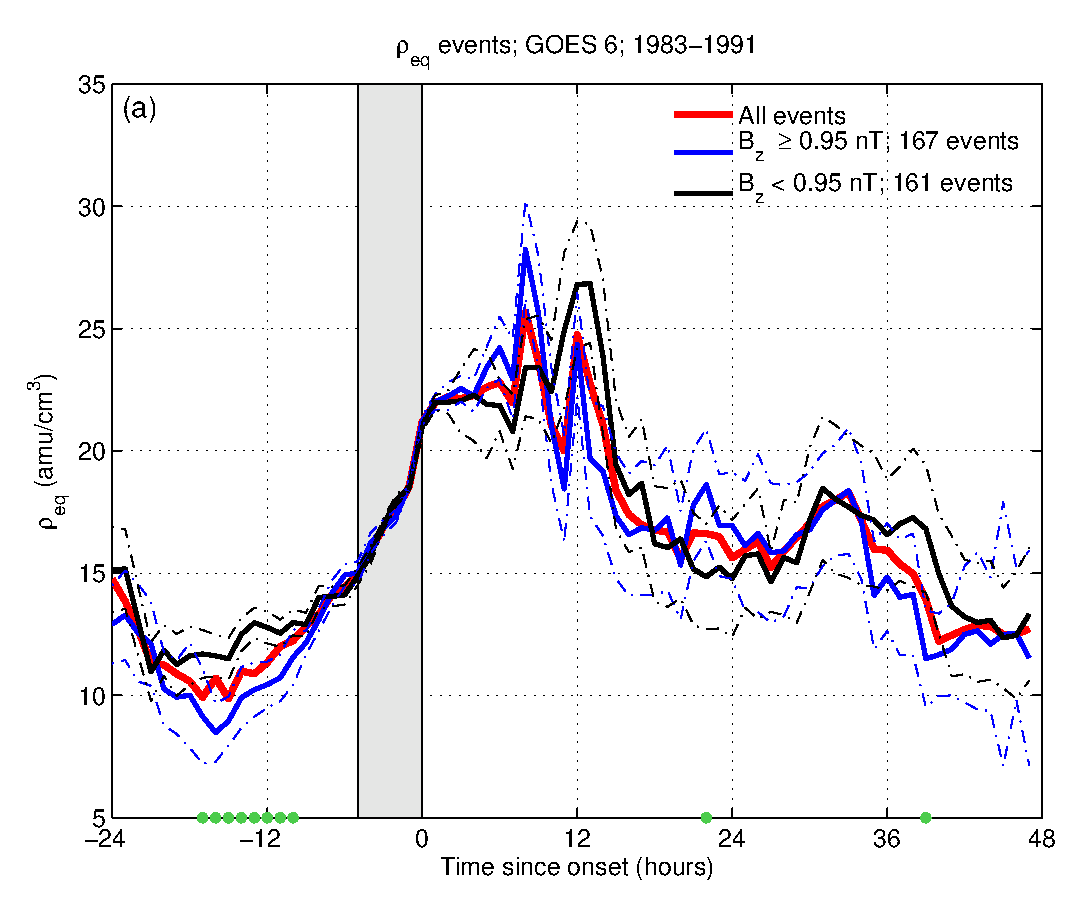
\includegraphics[width=0.7\linewidth]{Figures/RhoBinnedB_z-case24-t020-tf25-GOES6}
	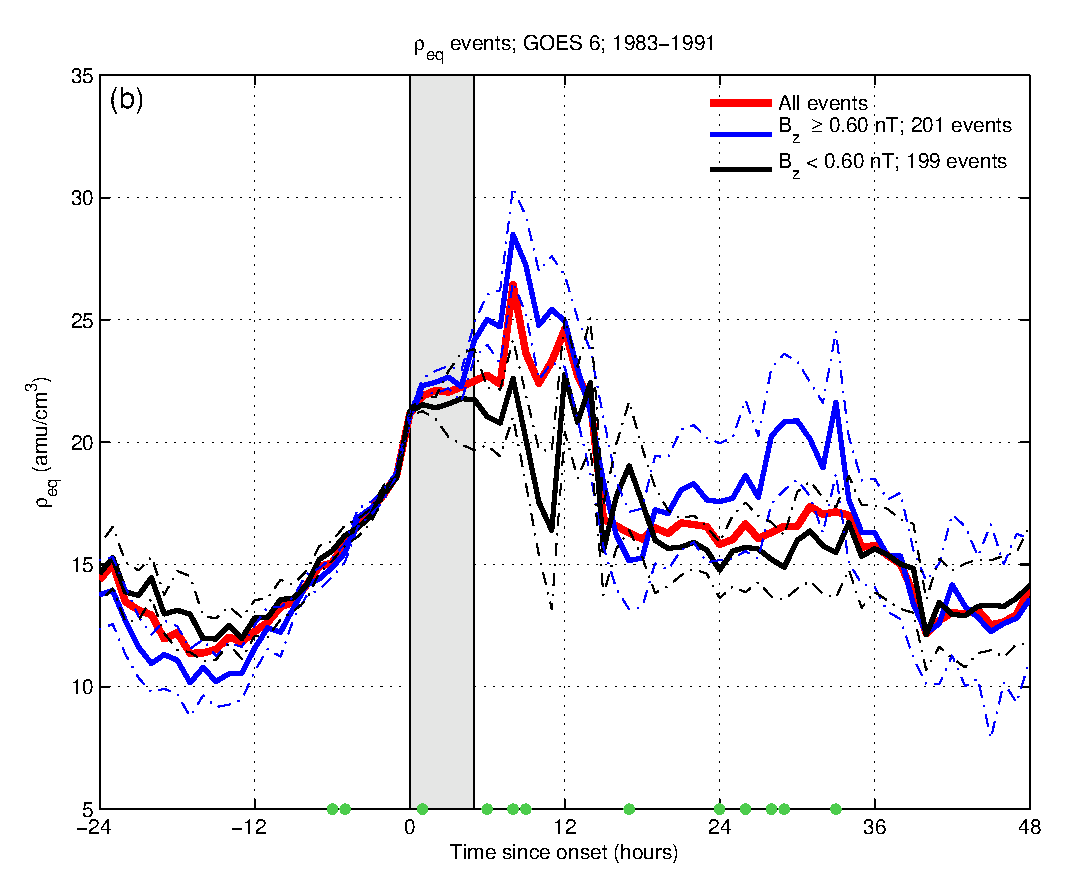
\includegraphics[width=0.7\linewidth]{Figures/RhoBinnedB_z-case24-t025-tf30-GOES6}	
	\caption{\req\ events binned by median $B_z$ before (top panel) and after (bottom panel) event onset.}
	\label{fig:RhoBinnedBz}
\end{figure}

For each binning method, a two sample t-test was performed for each hour to determine if the samples in each bin had significantly different medians from those of the other bin. As there are 73 hours to perform a t-test on, a 95\% confidence interval could be expected to have at least four randomly significant results. Because of this, the six significant t-test result for events binned by pre-onset $B_z$ can only barely confirm that such a division shows significantly different behaviors, whereas the nine significant test results for post-onset $B_z$, six of which are consecutive hours, can be said to show a more significant division in behavior between the bins. This physically suggests that the further into a \req\ increase you get, the more $B_z$ orientation impacts the long-term recovery to normal conditions (and indeed moving the window further in time did continue to show significance, but weakly and with no obvious trend). If instead of splitting into equal-number bins, the division is based on positive or negative $B_z$, either time window produces seven or more significant results, but with the added complication that one bin has twice as many samples as the other and may be biased by averaging or the lack thereof. 

\cite{Temerin2002NewModelPredictionDst} discuss the impact of $B_z$ on their model of \dst\ showing a seasonal variation of \dst. Figure \ref{fig:DoYDst} shows how \dst\ seems to vary with day of year (DoY) in our nonlinear models. These plots show a nonlinear model trained on all data, then predicted over a uniform grid of points to visualize the underlying structure of the model. The top panel predicts \dst\ using DoY as an input, showing the average model output over 40 ensemble models, along with the standard deviation at each point. The bottom panel predicts \dst\ using both DoY and $B_z$ as inputs, also using a 40-member ensemble average, but with the actual datapoints overlaid to give an idea of what the structure may be derived from. Marker size in this panel is based on the value of \dst\ at that point. It seems to support the idea of a seasonal variation, and weakly the idea that $B_z$ also plays a part in that relationship.


\begin{figure}[htp!]
	\centering
	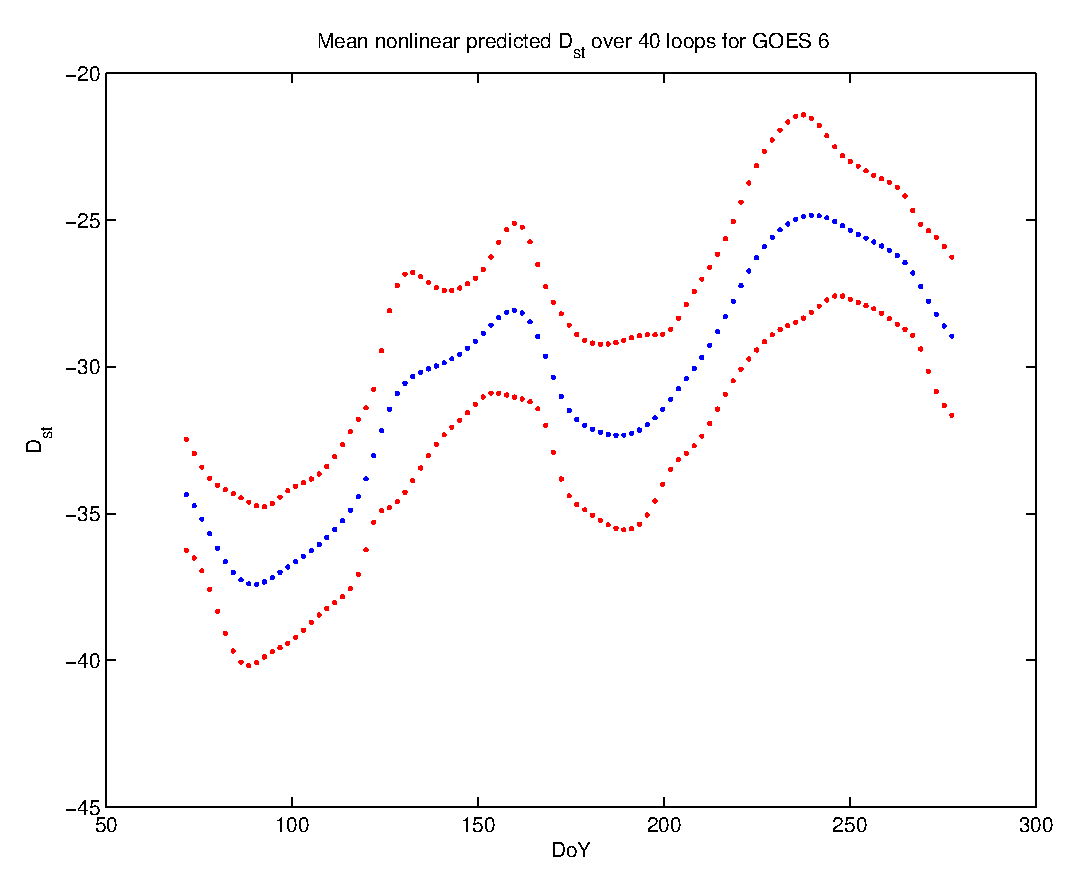
\includegraphics[width=0.7\linewidth]{Figures/NNDoY-Dst-GOES6}	
	\includegraphics[width=0.7\linewidth]{Figures/NNDoY-Bz-Dst-GOES6}
	\caption{Top: \dst\ predicted by nonlinear model of day of year. Bottom: Same, but including a dimension for $B_z$.}
	\label{fig:DoYDst}
\end{figure}

\section{Summary}
This chapter explored a number of linear and nonlinear models, in an effort to determine which solar wind and geomagnetic variables are most connected to the behavior of \req. While it was found that \f\ is most linearly correlated, it was also found that the other linear variables were highly collinear, providing little new information to the model when combined with \f.  It was also found that the correlations varied between different GOES satellites, as well as had a large variation in the nonlinear testing models. 

The epoch plots made to verify and extend the findings of \cite{Takahashi2010SolarCycleVariation} found that \req\ was significantly enhanced by an increase in geomagnetic activity on an hourly timescale, but was only weakly significant on a daily timescale. It also appears that this enhancement does not depend on the current condition of the interplanetary magnetic field $B_z$, but that high solar activity (via \f) does significantly influence the behavior of \req\ before and after a geomagnetic event, whether defined as an increase in \req\ or a decrease in \dst. Physically this suggests that active solar conditions act as a significant pre-requisite for processes that enhance plasma mass density around Earth during all detectable time periods.


